% vim: set tw=0:
\documentclass{beamer}
\usepackage{graphicx}
\usepackage{hyperref}
\hypersetup{pdfborder={0 0 0 0}}

% Reasonable themes:
% Antibes Bergen Berkeley Berlin Frankfurt Goettingen Ilmenau Luebeck Malmoe
% Montpellier PaloAlto Rochester Singapore Szeged Warsaw bars boxes
% compatibility default lined plain shadow sidebar split tree
% And these ones include the author's name on every slide:
% Berkeley

% Declare themes.
\mode<presentation>
\usetheme{UWHEP}

% Personal macros.
\newcommand{\email}[1]{{\texttt #1}}
\newcommand{\newframe}[1]{\section{#1}
    \frametitle{\sc{#1}}}
\newcommand{\subframe}[1]{\subsection{#1}
    \frametitle{\sc{#1}}}
\newcommand{\supers}[1]{\ensuremath{^\textrm{#1}}}
\newcommand{\subs}[1]{\ensuremath{_\textrm{#1}}}
\newcommand{\ca}{\ensuremath{\sim}}
\renewcommand{\email}[1]{\href{mailto:#1}{\nolinkurl{#1}}}

% Author information.
\title{T2 Status}
\author[Maier, Mohapatra]{
    Will Maier \and Ajit Mohapatra\\
    {\tt wcmaier@hep.wisc.edu}\\
    {\tt ajit@hep.wisc.edu}}
\institute[Wisconsin]{University of Wisconsin - High Energy Physics}
\date{2010.08.17}
\logo{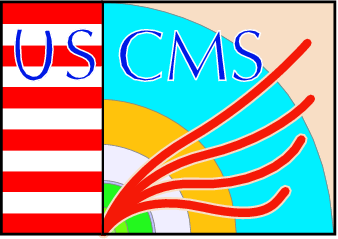
\includegraphics[height=0.6cm]{../../../Graphics/USCMS_logo.png}\hspace{.1cm}
\includegraphics[height=0.75cm]{../../../Graphics/UW_logo.png}}

\begin{document}

\begin{frame}
    \titlepage
\end{frame}

%\section{Overview}
%\begin{frame}
%    \tableofcontents
%\end{frame}

\section{Facilities}
\subsection{Software and Storage}
\begin{frame}
\frametitle{}

\begin{itemize}
    \item Deployed 28 2x8 core Opteron 6136 servers
    \begin{itemize}
        \item 4 didn't ship because they continued to fail burn in (just arrived)
        \item 4 more failed burn in on arrival; RMAing
        \item Otherwise, added storage and slots at the right time
    \end{itemize}
    \item Deployed Brian's xrootd redirector frontend
    \begin{itemize}
        \item Assuming it scales, would make switch to HDFS really easy here\ldots{}
    \end{itemize}
    \item Purchased 2x12 Opteron 6176 SE test server; should arrive soon for benchmarking
    \item Deployed tsar~\footnote{\url{http://code.hep.wisc.edu/tsar}} data service
    \item Debugging iowait spikes on PNFS headnode
    \begin{itemize}
        \item Strongly correlated with PNFS queue backups
        \item Tracking lots of system-level metrics in tsar
    \end{itemize}
    \item 2010.07.29: dCache filled up, chaos ensued
\end{itemize}
\end{frame}

\subsection{Production and Monitoring}
\begin{frame}
\frametitle{}

\begin{itemize}
    \item JobRobot: OK
    \item SAM: OK
    \item RSV: OK
    \item PhEDEx:
    \begin{itemize}
        \item Debug and Prod instances running stably with 3\_3\_1
        \item Fixed bug: DownloadVerify script ignored exit code from the FileDownload script; failed transfers marked successful in PhEDEX
    \end{itemize}
    \item MC Production:
    \begin{itemize}
        \item Summer10 continues along with some leftover Spring10 alpgens
        \item Fall10 started (38x) with some pre-production samples delivered already for validation
        \item Production of the Spring10 alpgens went well (with the usual issues) in the US during past 2 weeks

    \end{itemize}
\end{itemize}
\end{frame}

\end{document}
